\section{Arquitectura del Software}
El modelo de arquitectura 4+1 fue diseñado por Philippe Kruchten para poder describir la arquitectura de sistemas de software, basados en el uso de múltiples vistas, dichas vistas describen el sistema desde diferentes puntos de vista como de usuario final o desarrolladores. \\
Las cuatro vistas de este modelo son:
\begin{itemize}
	\item \textbf{Vista de Procesos:} Trata los aspectos dinámicos del sistema y como su nombre lo dice, explica todos los procesos del sistema y como es que se comunica el actor con el sistema.
	\item \textbf{Vista Lógica:} Enfocada a describir la estructura y funcionalidad de un sistema con ayuda de diagramas UML como Diagramas de Clase o de Secuencia.

	\item \textbf{Vista de Desarrollo:} Muestra el sistema desde el punto de vista de un programador. Se plasman las interfaces que se van a utilizar y el enlace entre cada una. Se utilizan Diagramas de Componentes o de Paquetes.
	\item \textbf{Vista Física:} Esta relacionado con la topología de componentes de hardware que se implementan para poder utilizar el sistema o aplicación. Muestra los componentes físicos como computadoras, redes, nodos, etc.
	\item \textbf{Vista de Escenarios:} Utilizando Casos de Uso, describe secuencias de interacciones entre objetos y procesos.
\end{itemize}

En la figura \ref{fig:Modelo de Arquitectura 4+1: Kruchten} nos muestra como es que se ha diseñado este modelo:
\begin{figure}[!h]
	\centering
	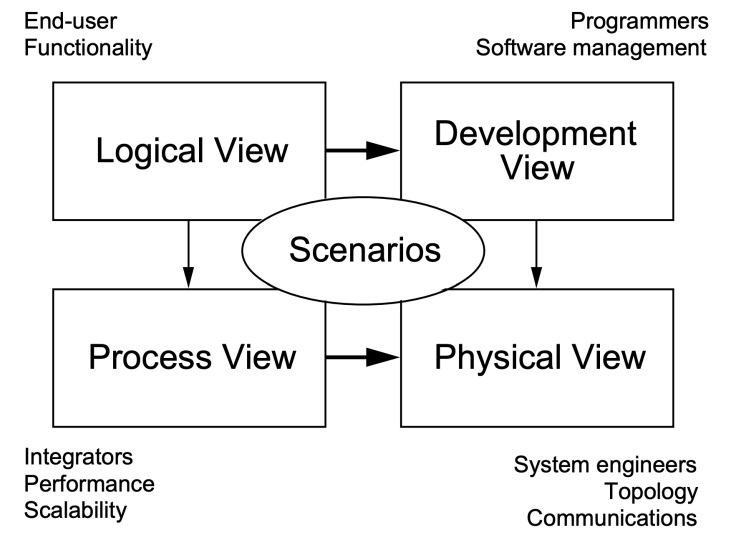
\includegraphics[width=1\textwidth]{./diseno/arquitectura/imagenes/arquitectura}
	\caption{Modelo de Arquitectura 4+1: Kruchten}
	\label{fig:Modelo de Arquitectura 4+1: Kruchten}
\end{figure}
